\section{Local fields and exchange--correlation kernels}\label{sec:4.6}

The absorption spectrum of silicon has two peaks, at 3.42 and \SI{4.24}{eV} (\cref{fig:4-siloss}), and its static screening saturates at $\varepsilon_\infty = 11.7$. A calculation that lets each electron respond on its own, with band energies fitted to experiment, puts the upper peak in nearly the right place, turns the lower one into a shoulder, and finds a dielectric constant within a few percent of 11.7. Adding the microscopic fields that the induced charge produces inside each cell lowers both peaks and lowers $\varepsilon_\infty$ by about a tenth. Adding the simplest exchange--correlation kernel undoes about half of that and barely changes the shape. Only the attraction between the excited electron and its hole, the subject of \cref{sec:4.9}, restores the lower peak. Each of these steps is a different approximation to the proper response $\tilde R$ of \cref{sec:4.4}. For dark matter the differences matter where the rate is largest for light masses: in the first few eV above the gap, where the loss function is small and the screening strong.

\subsection{The crystal bubble}

Take the Kohn--Sham states of \cref{sec:3.4}, with band energies $\varepsilon_{n\vect{k}}$ and occupations $f_{n\vect{k}}$ (\cref{eq:3.2-fnk}), as a system of independent electrons, and compute its density response matrix $R_{\vect{G}\vect{G}'}$ of \cref{eq:4.4-RGG} from the Lehmann representation \cref{eq:4.1-lehmann}. The steps are those of the electron gas in \cref{sec:4.5}, with Bloch states in place of plane waves. In the Bloch basis the density operator at $\vect{q} + \vect{G}'$ is \cref{eq:3.2-ne} with $\vect{q} \to \vect{q} + \vect{G}'$,
\begin{equation*}
  n_e(\vect{q}+\vect{G}') = \sum_s\sum_{\vect{k}}\sum_{mn}\rho_{mn}(\vect{k},\vect{q}+\vect{G}')\,c^\dagger_{m,\vect{k}+\vect{q},s}\,c_{n\vect{k}s} ,
\end{equation*}
with $\vect{q}$ in the first zone. The reciprocal vector does not change the crystal momentum of the final state, $\vect{k} + \vect{q} + \vect{G}' \equiv \vect{k} + \vect{q}$; it only changes the plane wave that probes the two states, through the density vertex $\rho_{mn}$ of \cref{eq:3.2-rho}. Acting on an occupation-number state $|i\rangle$ of Bloch states, the operator moves one electron from $n\vect{k}$ to $m,\vect{k}+\vect{q}$. In the resonant term of \cref{eq:4.1-lehmann} the final state is this move, with weight $f_{n\vect{k}}(1 - f_{m,\vect{k}+\vect{q}})$, energy $\varepsilon_{m,\vect{k}+\vect{q}} - \varepsilon_{n\vect{k}}$ and matrix elements $\langle f|n_e(\vect{q}+\vect{G}')|i\rangle = \rho_{mn}(\vect{k},\vect{q}+\vect{G}')$ and $\langle i|n_e(\vect{q}+\vect{G})^\dagger|f\rangle = \rho_{mn}(\vect{k},\vect{q}+\vect{G})^*$. In the antiresonant term the final state has the reverse move, from $m,\vect{k}+\vect{q}$ to $n\vect{k}$, with weight $f_{m,\vect{k}+\vect{q}}(1 - f_{n\vect{k}})$; its two matrix elements are the same pair, and its denominator $\omega + (\varepsilon_{n\vect{k}} - \varepsilon_{m,\vect{k}+\vect{q}}) + \ii0^+$ is the resonant one. As in the gas, the Pauli factors cancel in the sum of the two numerators, $f_{n\vect{k}}(1 - f_{m,\vect{k}+\vect{q}}) - f_{m,\vect{k}+\vect{q}}(1 - f_{n\vect{k}}) = f_{n\vect{k}} - f_{m,\vect{k}+\vect{q}}$, and the sum over the two spins gives the degeneracy factor $g_{\mathrm{deg}} = 2$.
\begin{keyresult}[Independent-particle bubble of a crystal]
\begin{equation}
  R^0_{\vect{G}\vect{G}'}(\vect{q},\omega) = \frac{g_{\mathrm{deg}}}{\Vol}\sum_{\vect{k}}\sum_{n,m}
  \bigl(f_{n\vect{k}} - f_{m,\vect{k}+\vect{q}}\bigr)\,
  \frac{\rho_{mn}(\vect{k},\vect{q}+\vect{G})^*\,\rho_{mn}(\vect{k},\vect{q}+\vect{G}')}{\omega + \varepsilon_{n\vect{k}} - \varepsilon_{m,\vect{k}+\vect{q}} + \ii0^+} ,
  \label{eq:4.6-R0}
\end{equation}
with $\Vol = N\Omega$, the sum over the $N$ crystal momenta of the first zone, and all pairs of bands. It is the density response at $\vect{q} + \vect{G}$ to a potential at $\vect{q} + \vect{G}'$ of electrons that move independently in the Kohn--Sham potential.
\end{keyresult}
This is the result of Adler and Wiser~\cite{adler1962quantum,wiser1963dielectric}, and it is \cref{eq:E.6-R0}, written there with a finite broadening. For one band of plane waves, $\rho_{mn} \to 1$ at $\vect{G} = \vect{G}' = 0$ and the matrix reduces to the bubble \cref{eq:4.5-R0} of the gas. In a crystal the off-diagonal elements do not vanish: a potential at $\vect{q}$ moves electrons into states whose overlap with the initial ones is modulated on the scale of the cell, and the induced density has components at every $\vect{q} + \vect{G}$.

At small $q$ the vertex at $\vect{G} = 0$ between different bands is the optical one, \cref{eq:3.2-optical}, $\rho_{cv}(\vect{k},\vect{q}) = \vect{q}\cdot\vect{v}_{cv}(\vect{k})/(\varepsilon_{c\vect{k}} - \varepsilon_{v\vect{k}})$, while the vertices at $\vect{G} \neq 0$ tend to the finite $\rho_{cv}(\vect{k},\vect{G})$. In an insulator at $T = 0$ only valence-to-conduction pairs contribute, with $f_{v\vect{k}} = 1$ and $f_{c\vect{k}} = 0$. Write $\Delta_{cv\vect{k}} = \varepsilon_{c\vect{k}} - \varepsilon_{v\vect{k}}$. The pairs $(n,m) = (v,c)$ and $(c,v)$ of \cref{eq:4.6-R0} give the head
\begin{equation}
  R^0_{\vect{0}\vect{0}}(\vect{q}\to0,\omega) = \frac{g_{\mathrm{deg}}q^2}{\Vol}\sum_{\vect{k}}\sum_{v,c}\frac{|\hat{\vect{q}}\cdot\vect{v}_{cv}(\vect{k})|^2}{\Delta_{cv\vect{k}}^2}
  \left[\frac{1}{\omega - \Delta_{cv\vect{k}} + \ii0^+} - \frac{1}{\omega + \Delta_{cv\vect{k}} + \ii0^+}\right] ,
  \label{eq:4.6-head}
\end{equation}
of order $q^2$, as \cref{app:D.7} requires of every proper response of an insulator. Its imaginary part, multiplied by $-v_{\mathrm{C}}(q) = -e^2/q^2$, is the absorptive part of the head of the dielectric matrix at positive frequency,
\begin{equation}
  \varepsilon_2^{\mathrm{IP}}(\omega) = \frac{\pi g_{\mathrm{deg}}e^2}{\Vol}\sum_{\vect{k}}\sum_{v,c}\frac{|\hat{\vect{q}}\cdot\vect{v}_{cv}(\vect{k})|^2}{\Delta_{cv\vect{k}}^2}\,\delta(\omega - \Delta_{cv\vect{k}}) ,
  \label{eq:4.6-eps2}
\end{equation}
where the label IP marks independent particles. It counts the vertical transitions at energy $\omega$, each weighted by its squared velocity matrix element along the field: this is the golden-rule absorption of light, through $\sigma_1 = \omega\varepsilon_2$ of \cref{eq:4.4-sigma}. The real part at $\omega = 0$ is
\begin{equation}
  \varepsilon_1^{\mathrm{IP}}(0) = 1 + \frac{2g_{\mathrm{deg}}e^2}{\Vol}\sum_{\vect{k}}\sum_{v,c}\frac{|\hat{\vect{q}}\cdot\vect{v}_{cv}(\vect{k})|^2}{\Delta_{cv\vect{k}}^3} ,
  \label{eq:4.6-static}
\end{equation}
since the bracket of \cref{eq:4.6-head} is $-2/\Delta_{cv\vect{k}}$ at $\omega = 0$. The third power of the transition energy makes the static screening sensitive to the smallest gaps. A Kohn--Sham gap that is too small therefore makes $\varepsilon_\infty$ too large, as the PBE value 13.04 against the measured 11.7 shows. The scissor of \cref{eq:3.4-scissor} leaves $\rho_{cv}$, and so the ratio $\vect{v}_{cv}/\Delta_{cv\vect{k}}$, unchanged (\cref{eq:3.4-vscis}). It then shifts $\varepsilon_2^{\mathrm{IP}}$ rigidly to higher energy and lowers \cref{eq:4.6-static}, whose terms go as $|\rho_{cv}/q|^2/\Delta_{cv\vect{k}}$.

In practice \cref{eq:4.6-R0} is summed on a grid of $\vect{k}$ points, over the occupied bands and a finite number of empty ones, with a broadening in place of $\ii0^+$ that must be larger than the spacing of the transition energies on the grid. The head and the wings, the elements with one index zero, are computed analytically in $\hat{\vect{q}}$ from velocity matrix elements, and the matrix is cut off at a finite number of reciprocal vectors.

\subsection{The random-phase approximation in a crystal}

The random-phase approximation of \cref{sec:4.5} replaces the proper response by the bubble, now as a matrix,
\begin{equation}
  \tilde R_{\vect{G}\vect{G}'} \simeq R^0_{\vect{G}\vect{G}'}, \qquad
  \varepsilon_{\vect{G}\vect{G}'} = \delta_{\vect{G}\vect{G}'} - v_{\mathrm{C}}(|\vect{q}+\vect{G}|)\,R^0_{\vect{G}\vect{G}'} ,
  \label{eq:4.6-rpa}
\end{equation}
with \cref{eq:4.4-epsGG}. Each electron responds as an independent particle to the total potential, external plus Hartree, at every $\vect{q} + \vect{G}$. The macroscopic function then comes at two levels. Keeping only the head gives $\varepsilon_{\mathrm{mac}} \simeq \varepsilon_{\vect{0}\vect{0}} = 1 - v_{\mathrm{C}}(q)R^0_{\vect{0}\vect{0}}$, the random-phase approximation without local fields. Inverting the whole matrix gives $\varepsilon_{\mathrm{mac}} = 1/(\varepsilon^{-1})_{\vect{0}\vect{0}}$, the random-phase approximation with local fields, which by \cref{eq:D.7-macbar} is
\begin{equation}
  \varepsilon_{\mathrm{mac}} = 1 - v_{\mathrm{C}}(q)\,\bar R_{\vect{0}\vect{0}}, \qquad \bar R = R^0 + R^0\,\bar v\,\bar R ,
  \label{eq:4.6-rpaLF}
\end{equation}
with $\bar v$ the Coulomb matrix without its element at $\vect{G} = 0$. In this form the singular head of $v_{\mathrm{C}}$ never appears in the inversion, and the limit $\vect{q} \to 0$ is taken in $R^0$ alone (\cref{app:D.7}).

Since $v_{\mathrm{C}}$ is real, the imaginary part of $\varepsilon_{\vect{0}\vect{0}}$ is \cref{eq:4.6-eps2} exactly: without local fields the random-phase approximation has the absorption spectrum of independent particles. Screening enters through the real part, and so through the loss function $L = \varepsilon_2/|\varepsilon|^2$ of \cref{sec:4.4}, which it suppresses by $|\varepsilon|^2$ wherever $\varepsilon_1$ is large. Going from independent particles to this level changes the rate, through $1/|\varepsilon|^2$, and leaves the optical spectrum unchanged. The local fields are the first correction that changes $\varepsilon_2$.

The local fields have a classical analog. A capacitor filled with layers of different dielectric constants, stacked along the field, has a uniform $D$ and a field $E = D/\varepsilon(x)$ that varies from layer to layer. The capacitance measures the average field, $\langle E\rangle = D\langle1/\varepsilon\rangle$, so the effective constant is $1/\langle1/\varepsilon\rangle$, the harmonic mean, which is never larger than the arithmetic mean $\langle\varepsilon\rangle$. The macroscopic function \cref{eq:4.4-epsmac} has exactly this structure: it is the inverse of the average of the inverse, while the head $\varepsilon_{\vect{0}\vect{0}}$ is the average itself. In silicon the polarizable charge lies in the bonds. A uniform field pushes it along the bonds, the displaced charge forms dipoles on the scale of the cell, and their microscopic Hartree field, at $\vect{G} \neq 0$, points against the applied field in the regions where the polarizable electrons are. The electrons feel less than the average field, and the crystal screens less than the head alone predicts. The two would agree if the induced density were uniform, as in the gas, and they disagree most where the response is concentrated in a small part of the cell.

\Cref{fig:4-si-approx} shows the consequence for silicon in a model calculation with the empirical pseudopotential of Cohen and Bergstresser (\cref{sec:3.3}), whose form factors were fitted to measured transition energies; no scissor is needed. The independent-particle spectrum, panel (a), has its upper peak at \SI{4.26}{eV}, close to the measured \SI{4.24}{eV}, with a height of 41 against the measured 46. At \SI{3.42}{eV}, where the measured spectrum has its lower peak of height 36, the model has only 15, a shoulder. The local fields lower the upper peak to 34 and move it to \SI{4.32}{eV}; at \SI{3.42}{eV} they leave 13. Spectral weight moves up, as the f-sum rule with local fields (\cref{app:D.7}) requires if the low-energy peaks lose some, and the agreement with experiment gets worse. The same happens in first-principles calculations on top of quasiparticle bands~\cite{albrecht1998ab}. Since the static constant is the inverse moment $1 + (2/\pi)\int\varepsilon_2/\omega$ (\cref{eq:4.4-inverse}), weight moved up lowers it, and the local fields lower $\varepsilon_\infty$ (\cref{we:4-siepsinf}).

\begin{figure}[tbp]
  \centering
  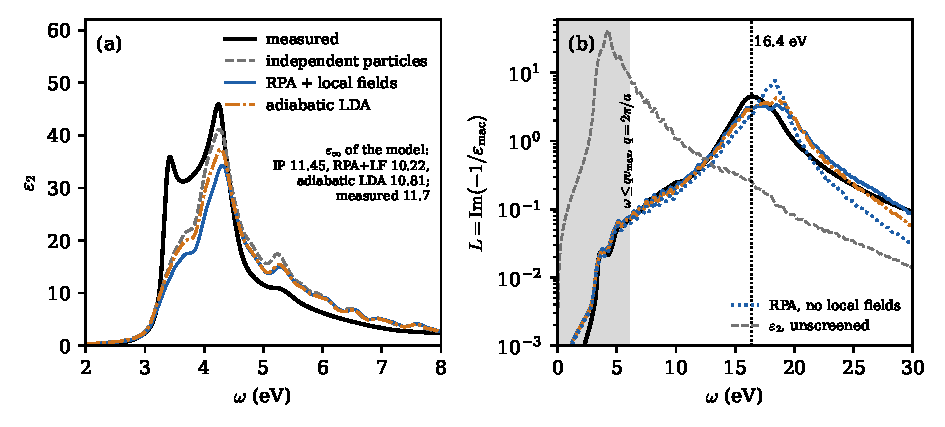
\includegraphics[width=\linewidth]{figures/ch04/fig4_7.pdf}
  \caption{Three many-body approximations to the dielectric function of crystalline silicon at $\vect{q} \to 0$, in a model calculation. Band energies and Bloch states come from the local empirical pseudopotential of Cohen and Bergstresser~\cite{cohen1966band}, fitted to measured transition energies (no scissor shift). The sums run over a shifted $20^3$ grid of $\vect{k}$ points over the full zone, with 4 valence and 26 conduction bands, a local-field matrix of the 59 shortest reciprocal vectors, and a Lorentzian broadening of \SI{0.10}{eV}. The exchange--correlation kernel is the adiabatic local-density one, evaluated on the model's valence density with the Perdew--Zunger correlation energy~\cite{perdew1981self}. Black: measured at \SI{300}{K}~\cite{franta2017temperature}; panel (a) lists the static limits of the three approximations against the measured $\varepsilon_\infty = 11.7$ (\cref{sec:4.4}). (a) Absorptive part $\varepsilon_2$: independent particles (dashed gray), which is also the random-phase approximation without local fields; the random-phase approximation with local fields (solid blue); adiabatic LDA (dash-dotted orange). The strength of the measured lower peak at \SI{3.42}{eV} comes from the electron--hole attraction (\cref{sec:4.9}), and all three underestimate it. (b) Loss function on a logarithmic scale: the random-phase approximation without local fields (dotted blue), with local fields (solid blue), and adiabatic LDA (dash-dotted orange). Dashed gray: the unscreened $\varepsilon_2$ of independent particles, which a rate without screening would use in place of $L$. The model's loss peak lies about \SI{2}{eV} above the measured \SI{16.4}{eV} (dotted line), because its high conduction bands are not fitted. Shaded: energies up to $qv_{\mathrm{max}} = \SI{6.05}{eV}$ at a momentum transfer of one reciprocal-lattice unit, $q = 2\pi/a$, the range that dark matter of any mass can reach there.}
  \label{fig:4-si-approx}
\end{figure}

Panel (b) shows the loss function that sets the dark-matter rate. Up to about \SI{6}{eV} the loss function lies two to three orders of magnitude below the unscreened $\varepsilon_2$; this is the factor $1/|\varepsilon|^2$ that the head of the dielectric matrix already contains. On this scale the local fields are a correction of tens of percent. Between 3 and \SI{12}{eV} they raise $L$ by 10 to 35 percent, because they lower $|\varepsilon|$, and they cut the height of the plasmon peak from 7.6 to 3.4. A dark-matter rate integrates the loss function over $\vect{q}$ and over $\omega$ up to $qv_{\mathrm{max}}$, and for silicon and germanium the difference between rates computed with and without local fields is small~\cite{knapen2021dark}. Local fields matter more at momentum transfers of a few reciprocal vectors, where the off-diagonal elements of $R^0$ are as large as the diagonal ones, and at energies where semicore shells, localized near the nuclei, contribute.

Local fields have a second reading, which \cref{sec:4.9} uses. In the space of electron--hole pairs, the microscopic Hartree potential $\bar v$ is the bare Coulomb interaction between a pair and another pair at the same total momentum, with the long-range term at $\vect{G} = 0$ removed. This is the exchange kernel $K^{\mathrm{x}}$ of the Bethe--Salpeter equation. The random-phase approximation with local fields is that equation with the electron--hole attraction switched off, and it cannot bind an exciton.

\subsection{Time-dependent density-functional theory}

The bubble \cref{eq:4.6-R0} is built from Kohn--Sham states, and until now that was a convenience: the states of some independent-particle model were needed, and these were at hand. Time-dependent density-functional theory makes the choice exact. Runge and Gross proved that the time-dependent density of an interacting system, evolving from its ground state, determines the time-dependent external potential up to a function of time alone~\cite{runge1984density}. It follows, as in the static theory, that a system of independent electrons in a suitable time-dependent Kohn--Sham potential has the same density at all times. That potential is the external one plus the Hartree potential plus an exchange--correlation potential $v_{\mathrm{xc}}(\vect{r},t)$, which now depends on the density at all earlier times.

Linear response follows in three lines. A weak external potential energy $\phi_{\mathrm{ext}}$ changes the Kohn--Sham potential by
\begin{equation*}
  \delta V_{\mathrm{KS}}(\vect{r},t) = \phi_{\mathrm{ext}}(\vect{r},t) + \int\dd^3r'\,v_{\mathrm{C}}(\vect{r} - \vect{r}')\,\delta\nd(\vect{r}',t)
  + \int\dd^3r'\int\dd t'\,f_{\mathrm{xc}}(\vect{r},\vect{r}',t - t')\,\delta\nd(\vect{r}',t') ,
\end{equation*}
where the exchange--correlation kernel
\begin{equation}
  f_{\mathrm{xc}}(\vect{r},\vect{r}',t - t') = \frac{\delta v_{\mathrm{xc}}(\vect{r},t)}{\delta\nd(\vect{r}',t')}\bigg|_{\nd_{\mathrm{gs}}} ,
  \label{eq:4.6-fxc}
\end{equation}
is the functional derivative taken at the ground-state density $\nd_{\mathrm{gs}}$. Since the Kohn--Sham electrons are independent, their density responds to their own potential through the bubble: $\delta\nd = R^0\,\delta V_{\mathrm{KS}}$, with $R^0$ of \cref{eq:4.6-R0}. And $\delta\nd$ is, by construction, the density change of the interacting system, $\delta\nd = R\,\phi_{\mathrm{ext}}$. In reciprocal space, with $f_{\mathrm{Hxc}} = v_{\mathrm{C}} + f_{\mathrm{xc}}$ the matrix $(f_{\mathrm{Hxc}})_{\vect{G}\vect{G}'} = v_{\mathrm{C}}(|\vect{q}+\vect{G}|)\delta_{\vect{G}\vect{G}'} + (f_{\mathrm{xc}})_{\vect{G}\vect{G}'}(\vect{q},\omega)$, the two statements combine to $R\phi_{\mathrm{ext}} = R^0(\phi_{\mathrm{ext}} + f_{\mathrm{Hxc}}R\phi_{\mathrm{ext}})$ for every $\phi_{\mathrm{ext}}$.
\begin{keyresult}[Dyson equation of time-dependent density-functional theory]
\begin{equation}
  R = R^0 + R^0 f_{\mathrm{Hxc}} R, \qquad \tilde R = R^0 + R^0 f_{\mathrm{xc}}\tilde R ,
  \label{eq:4.6-tddft}
\end{equation}
as matrices in the reciprocal-lattice vectors at fixed $(\vect{q},\omega)$. With the exact kernel, $R$ is the exact density response, although $R^0$ is built from Kohn--Sham states. The random-phase approximation is $f_{\mathrm{xc}} = 0$.
\end{keyresult}
The proper response follows from the first form by splitting off the Coulomb kernel, since $R = \tilde R + \tilde Rv_{\mathrm{C}}R$ (\cref{eq:4.4-dyson}) has the solution $\tilde R = (1 - R^0f_{\mathrm{xc}})^{-1}R^0$. This is \cref{eq:E.6-dyson}, and Petersilka, Gossmann and Gross used it to compute excitation energies as the poles of $R$~\cite{petersilka1996excitation}. For the macroscopic function, the kernel of \cref{eq:4.6-rpaLF} becomes $\bar v + f_{\mathrm{xc}}$, with the long-range Coulomb term still removed.

The exact kernel, however, is unknown. The Kohn--Sham gap is smaller than the true one (\cref{sec:3.4}), and the poles of $R^0$ lie at the wrong energies; the kernel must move them. It must also bind the electron and the hole into excitons, which takes an attraction of long range. Both are hard to get from a function of the density at one point.

The most widely used kernel is the \emph{adiabatic local-density approximation} (ALDA). It takes the exchange--correlation potential of \cref{eq:3.4-LDA} at the instantaneous local density, so that the kernel is local in space and instantaneous in time~\cite{gross1985local},
\begin{equation}
  f_{\mathrm{xc}}^{\mathrm{ALDA}}(\vect{r},\vect{r}',t - t') = \delta(\vect{r} - \vect{r}')\,\delta(t - t')\,\frac{\dd^2\bigl[\nd\,\varepsilon_{\mathrm{xc}}(\nd)\bigr]}{\dd\nd^2}\bigg|_{\nd_{\mathrm{gs}}(\vect{r})} .
  \label{eq:4.6-alda}
\end{equation}
It is negative, since exchange and correlation make the potential more attractive where the density grows. In reciprocal space it is a function of $\vect{G} - \vect{G}'$ alone and does not depend on $\vect{q}$ or $\omega$.

These properties fix what the kernel misses. Being instantaneous, it has no frequency dependence and cannot open the gap: the absorption edge stays at the Kohn--Sham gap, and a scissor or quasiparticle energies are still needed. Being local, its matrix is finite as $\vect{q} \to 0$. In the optical limit the head element enters $\tilde R_{\vect{0}\vect{0}}$ multiplied by $R^0_{\vect{0}\vect{0}} = O(q^2)$ and drops out, and the wings drop out with one power of $q$. The kernel acts only through the body of the matrix, at $\vect{G}, \vect{G}' \neq 0$, alongside $\bar v$, which it partly cancels. An exciton, however, needs the attraction between an electron and a hole at large separation, which in an insulator behaves as $-\alpha_{\mathrm{xc}}/|\vect{q}+\vect{G}|^2$ in reciprocal space~\cite{reining2002excitonic}; a local kernel has no such term. In \cref{fig:4-si-approx} the adiabatic LDA spectrum lies between the two random-phase ones and close to the one with local fields, with the upper peak at a height of 37, and its static constant lies between theirs (\cref{we:4-siepsinf}). Its lower peak is as weak as theirs. This is the general finding for semiconductors: for absorption the adiabatic LDA is little better than the random-phase approximation with local fields, and for energy-loss spectra it does well because the random-phase approximation already does~\cite{onida2002electronic,botti2007time}.

\subsection{Local-field factor of the electron gas}

In the homogeneous gas every matrix is diagonal, and \cref{eq:4.6-tddft} gives $\tilde R = R^0/(1 - f_{\mathrm{xc}}R^0)$ with the Lindhard function $R^0$ of \cref{eq:4.5-lindhard}. The many-body literature on the gas writes the same proper response with a static \emph{local-field factor} $G_{\mathrm{LF}}(q)$. It is defined by
\begin{equation*}
  \varepsilon(q,\omega) = 1 - \frac{v_{\mathrm{C}}(q)\,R^0(q,\omega)}{1 + v_{\mathrm{C}}(q)\,G_{\mathrm{LF}}(q)\,R^0(q,\omega)} .
\end{equation*}
An electron feels the Hartree potential of the induced density reduced by the factor $1 - G_{\mathrm{LF}}$, because the exchange--correlation hole keeps the other electrons away from it. The name is the gas analog of the local fields of a crystal: in both cases the field an electron actually feels differs from the average one. Comparing with $\varepsilon = 1 - v_{\mathrm{C}}R^0/(1 - f_{\mathrm{xc}}R^0)$,
\begin{equation}
  f_{\mathrm{xc}}(q) = -v_{\mathrm{C}}(q)\,G_{\mathrm{LF}}(q) = -\frac{e^2}{q^2}\,G_{\mathrm{LF}}(q) .
  \label{eq:4.6-GLF}
\end{equation}
A static local-field factor is thus a static kernel, and every model of $G_{\mathrm{LF}}$ in the literature on the gas~\cite[Chap.~5]{giuliani2005quantum} is a kernel of time-dependent density-functional theory for it.

The long-wavelength limit is fixed by thermodynamics. A static potential of long wavelength shifts the local chemical potential, as in the Thomas--Fermi argument of \cref{sec:4.4}, and the proper response is $\tilde R(q\to0,0) = -\partial\nd_e/\partial\mu_{\mathrm{ch}}$, with $\mu_{\mathrm{ch}}$ the chemical potential without the Hartree term. With $R^0(q\to0,0) = -2\mathcal{N}_{\mathrm{F}}$, the inverse of $\tilde R = R^0/(1 - f_{\mathrm{xc}}R^0)$ is
\begin{equation}
  \frac{\partial\mu_{\mathrm{ch}}}{\partial\nd_e} = \frac{1}{2\mathcal{N}_{\mathrm{F}}} + f_{\mathrm{xc}}(q\to0) ,
  \label{eq:4.6-compress}
\end{equation}
which is the compressibility sum rule: the kernel at long wavelength is the second derivative of the exchange--correlation energy density, $\dd^2(\nd\varepsilon_{\mathrm{xc}})/\dd\nd^2$. The adiabatic LDA satisfies it by construction. For exchange alone, $v_{\mathrm{x}} = \tfrac43\varepsilon_{\mathrm{x}} \propto \nd^{1/3}$ with $\varepsilon_{\mathrm{x}} = -3e^2k_{\mathrm{F}}/16\pi^2$, so $f_{\mathrm{x}} = \dd v_{\mathrm{x}}/\dd\nd = v_{\mathrm{x}}/3\nd$, and with $\nd = k_{\mathrm{F}}^3/3\pi^2$,
\begin{equation*}
  f_{\mathrm{x}} = -\frac{e^2}{4k_{\mathrm{F}}^2}, \qquad G_{\mathrm{LF}}(q) = \frac{q^2}{4k_{\mathrm{F}}^2}\quad (q \ll k_{\mathrm{F}}) .
\end{equation*}
Correlation adds to this. At $r_s = 2$, the Perdew--Zunger correlation energy~\cite{perdew1981self} raises the coefficient from $\tfrac14$ to 0.267, and \cref{eq:4.6-compress} with $k_{\mathrm{TF}}^2/k_{\mathrm{F}}^2 = 1.33$ (\cref{sec:4.5}) says that the gas is 1.55 times more compressible than free electrons of the same density. An electron surrounded by its exchange--correlation hole repels the others less, the gas yields more easily to a slow potential, and it screens more strongly than the random-phase approximation says.

The adiabatic LDA fails at short wavelengths, where dark matter scatters. Its $G_{\mathrm{LF}} = 0.267\,q^2/k_{\mathrm{F}}^2$ grows without bound, while the factor of the real gas follows the $q^2$ law only for $q \ll k_{\mathrm{F}}$; beyond $q \sim k_{\mathrm{F}}$ it stops growing and stays of order one~\cite[Chap.~5]{giuliani2005quantum}. At the typical momentum transfer $q_0 = \SI{3.73}{keV}$, which is $1.04\,k_{\mathrm{F}}$ at the silicon valence density, the local kernel is at the edge of its range of validity. There its factor is 0.29, and it raises the static Lindhard value $\varepsilon(q_0,0) = 2.10$ of \cref{sec:4.5} to 2.62. The correction to the screening at $q_0$ is thus of order a quarter. Its sign is reliable, its size at $q \sim k_{\mathrm{F}}$ only to the extent that the local kernel is.

\subsection{Many-body spread as an error measure}

Independent particles, the random-phase approximation with the head alone, the same with local fields, and an exchange--correlation kernel on top form a hierarchy, which the Bethe--Salpeter equation of \cref{sec:4.9} completes. The hierarchy is not an expansion in a small number: each level adds a physical effect whose size depends on the material, the energy and the momentum, so no level bounds the error of the one below. The hierarchy does measure how much a quantity depends on the many-body treatment. In silicon the static constant changes by about a tenth across the approximations of \cref{fig:4-si-approx} (\cref{we:4-siepsinf}), and the screening factor $1/\varepsilon_\infty^2$ at small $q$ by about a quarter. Near the gap, where excitons move weight, the spread is larger, and only the Bethe--Salpeter equation captures the shape of the spectrum there. Well above the gap, at the energies that hold most of the f-sum, the approximations agree to within the accuracy of the bands. This many-body spread, computed with the same bands, $\vect{k}$ grid and cutoffs in every approximation, is the many-body part of the theory uncertainty of a loss function. For heavier dark matter, whose rate is dominated by energies of several eV, it is small. For light dark matter, which deposits at most $\tfrac12\mchi v_{\mathrm{max}}^2$ (\cref{eq:1.3-omegamax}) and so samples the first eV above the gap, it is the leading part.

\begin{workedexample}{The local-field reduction of the dielectric constant of silicon}\label{we:4-siepsinf}
The calculation of \cref{fig:4-si-approx} yields the static limit of each approximation at $\vect{q} \to 0$ from the same states, from \cref{eq:4.6-static} for independent particles and from \cref{eq:4.6-rpaLF,eq:4.6-tddft} at $\omega = 0$ for the others. Independent particles, and equally the random-phase approximation without local fields, give $\varepsilon_\infty = 11.45$, within 2 percent of the measured 11.7. The small difference is a property of the model, whose form factors were fitted to measured transition energies. With the local fields of the 59 shortest reciprocal vectors, $\varepsilon_\infty = 10.22$, unchanged to three digits with 113 vectors; the local fields lower the dielectric constant by 11 percent. The adiabatic LDA kernel raises it again to 10.81, 6 percent above the random-phase value with local fields, so that it cancels about half of the local-field reduction. All three are converged in the $\vect{k}$ grid to better than 0.1 percent.

The PBE value 13.04 of \cref{sec:3.4} is a static linear-response calculation with Kohn--Sham bands, local fields and the adiabatic PBE kernel: it is the third of our approximations, with Kohn--Sham energies in place of fitted ones. It lies above the measured value by 11 percent, and the reason is \cref{eq:4.6-static}. The PBE gap is about half the measured one, and the static sum weights small transition energies by their inverse cube. The same representative PBE setting as \cref{app:E.1}, at the measured lattice constant on a $20^3$ grid, gives the other two approximations as well: 13.61 for independent particles and 12.20 with local fields, against 13.04 with the PBE kernel. The first-principles values follow the trend of the model values 11.45, 10.22 and 10.81: the local fields lower $\varepsilon_\infty$ by 10 percent, and the kernel restores part of it. Independent particles with fitted energies happen to land close to experiment, but the adiabatic kernel with fitted energies does not: at 10.81 it is 8 percent below 11.7. The adiabatic kernel lacks the electron--hole attraction, which lowers the energies of the transitions near the gap and so raises $\varepsilon_\infty$ (\cref{sec:4.9}).

For a dark-matter rate at momentum transfers small enough that $L \simeq \varepsilon_2/\varepsilon_\infty^2$, the local-field reduction of $\varepsilon_\infty$ alone changes the screening factor by $(11.45/10.22)^2 \simeq 1.25$. The kernel undoes part of it, and the electron--hole attraction more than makes up the rest.
\end{workedexample}
